\documentclass[12pt,a4paper,oneside]{report}

% FallGuard AI - full technical report.
% Compile from the repository root with:
%   xelatex -interaction=nonstopmode -halt-on-error -output-directory=output/pdf docs/FallGuard_AI_Full_Report.tex
% Run the command twice so the table of contents and references are updated.

\usepackage[a4paper,top=2.3cm,bottom=2.3cm,left=2.7cm,right=2.2cm,headheight=15pt]{geometry}
\usepackage{fontspec}
\setmainfont{Times New Roman}
\setsansfont{Arial}
\setmonofont{Consolas}
\XeTeXlinebreaklocale "vi"
\XeTeXlinebreakskip=0pt plus 1pt

\usepackage{amsmath,amssymb}
\usepackage{graphicx}
\usepackage{booktabs,longtable,tabularx,array,multirow}
\usepackage{enumitem}
\usepackage{fancyhdr}
\usepackage{titlesec}
\usepackage{xcolor}
\usepackage{hyperref}
\usepackage{bookmark}
\usepackage{float}
\usepackage{caption}
\usepackage{listings}
\usepackage{tikz}
\usetikzlibrary{arrows.meta,positioning,shapes.geometric,fit,calc}
\usepackage{pgfplots}
\pgfplotsset{compat=1.18}
\usepackage[most]{tcolorbox}
\usepackage{setspace}
\usepackage{microtype}

\definecolor{fgNavy}{HTML}{0B1F33}
\definecolor{fgBlue}{HTML}{1363DF}
\definecolor{fgCyan}{HTML}{17A2B8}
\definecolor{fgGreen}{HTML}{22A06B}
\definecolor{fgMint}{HTML}{DDF8EE}
\definecolor{fgRed}{HTML}{D64545}
\definecolor{fgOrange}{HTML}{E58A1F}
\definecolor{fgGray}{HTML}{52606D}
\definecolor{fgLight}{HTML}{F3F6F9}
\definecolor{fgLine}{HTML}{CED7E0}

\hypersetup{
  colorlinks=true,
  linkcolor=fgBlue,
  urlcolor=fgCyan,
  citecolor=fgGreen,
  pdftitle={FallGuard AI - Tài liệu mô tả toàn bộ dự án},
  pdfauthor={FallGuard Capstone Team},
  pdfsubject={Phát hiện té ngã thời gian thực bằng pose estimation và mô hình tuần tự}
}

\titleformat{\chapter}[display]
  {\bfseries\color{fgNavy}}
  {\filleft\Large Chương \thechapter}
  {0.5ex}
  {\titlerule\vspace{1ex}\Huge}
\titleformat{\section}{\Large\bfseries\color{fgNavy}}{\thesection}{0.7em}{}
\titleformat{\subsection}{\large\bfseries\color{fgBlue}}{\thesubsection}{0.7em}{}

\pagestyle{fancy}
\fancyhf{}
\fancyhead[L]{\small FallGuard AI}
\fancyhead[R]{\small Tài liệu kỹ thuật toàn hệ thống}
\fancyfoot[C]{\thepage}
\renewcommand{\headrulewidth}{0.4pt}
\setlength{\parindent}{1.1cm}
\setlength{\parskip}{0.35em}
\onehalfspacing

\newcolumntype{Y}{>{\raggedright\arraybackslash}X}
\newcommand{\code}[1]{\texttt{#1}}
\newcommand{\pathcode}[1]{\texttt{\detokenize{#1}}}
\newcommand{\important}[1]{\textbf{\color{fgRed}#1}}

\newtcolorbox{summarybox}[1][]{
  enhanced,breakable,colback=fgLight,colframe=fgBlue,
  boxrule=0.8pt,arc=2mm,left=3mm,right=3mm,top=2mm,bottom=2mm,
  title={#1},fonttitle=\bfseries,coltitle=white,colbacktitle=fgBlue
}
\newtcolorbox{warningbox}[1][]{
  enhanced,breakable,colback=yellow!8,colframe=fgOrange,
  boxrule=0.8pt,arc=2mm,left=3mm,right=3mm,top=2mm,bottom=2mm,
  title={#1},fonttitle=\bfseries,coltitle=white,colbacktitle=fgOrange
}
\newtcolorbox{resultbox}[1][]{
  enhanced,breakable,colback=fgMint,colframe=fgGreen,
  boxrule=0.8pt,arc=2mm,left=3mm,right=3mm,top=2mm,bottom=2mm,
  title={#1},fonttitle=\bfseries,coltitle=white,colbacktitle=fgGreen
}

\lstdefinestyle{fallguard}{
  basicstyle=\ttfamily\small,
  backgroundcolor=\color{fgNavy},
  basicstyle=\ttfamily\small\color{white},
  keywordstyle=\color{cyan!70},
  commentstyle=\color{green!60},
  stringstyle=\color{yellow!70},
  breaklines=true,
  columns=fullflexible,
  keepspaces=true,
  showstringspaces=false,
  frame=single,
  rulecolor=\color{fgNavy},
  xleftmargin=0.4em,
  xrightmargin=0.4em,
  aboveskip=0.8em,
  belowskip=0.8em
}
\lstset{style=fallguard}

\begin{document}

\begin{titlepage}
\pagecolor{fgNavy}
\color{white}
\begin{center}
  \vspace*{1.1cm}
  {\sffamily\Large ĐỒ ÁN CAPSTONE 2\par}
  \vspace{1.6cm}
  {\sffamily\bfseries\fontsize{32}{38}\selectfont FALLGUARD AI\par}
  \vspace{0.4cm}
  {\sffamily\Large Hệ thống phát hiện té ngã thời gian thực\par}
  \vspace{0.2cm}
  {\sffamily\large dựa trên ước lượng tư thế và mô hình chuỗi thời gian\par}
  \vspace{1.3cm}
  \begin{tcolorbox}[width=0.86\textwidth,colback=fgNavy!85!black,colframe=fgCyan,
      coltext=white,boxrule=1.2pt,arc=3mm]
  \centering
  \textbf{TÀI LIỆU MÔ TẢ TOÀN BỘ DỰ ÁN}\par
  \vspace{0.3cm}
  Dữ liệu $\rightarrow$ tiền xử lý $\rightarrow$ AI $\rightarrow$ xác minh sự kiện
  $\rightarrow$ webcam/web $\rightarrow$ cảnh báo Telegram
  \end{tcolorbox}
  \vfill
  \begin{tabular}{rl}
    \textbf{Sinh viên:} & \rule{8cm}{0.4pt} \\
    \textbf{Mã số sinh viên:} & \rule{8cm}{0.4pt} \\
    \textbf{Giảng viên hướng dẫn:} & \rule{8cm}{0.4pt} \\
    \textbf{Đơn vị:} & \rule{8cm}{0.4pt}
  \end{tabular}
  \vfill
  {\sffamily Phiên bản tài liệu: 1.0 - Tháng 09/2026\par}
\end{center}
\end{titlepage}
\nopagecolor
\color{black}

\pagenumbering{roman}
\chapter*{Tóm tắt}
\addcontentsline{toc}{chapter}{Tóm tắt}

FallGuard AI là một hệ thống phát hiện té ngã end-to-end từ camera, được xây dựng
cho đồ án Capstone 2. Hệ thống không phân loại độc lập từng ảnh. Thay vào đó, nó
trích xuất 33 điểm khớp cơ thể bằng MediaPipe Pose, chuẩn hóa theo tâm hông và
chiều dài thân, tạo chuỗi đặc trưng chuyển động, sau đó dùng mô hình tuần tự nhân
quả GRU để dự đoán đồng thời tư thế và xác suất sự kiện té ngã. Một state machine
tiếp tục kiểm tra tư thế nằm, thời gian bất động, sự hồi phục và thời gian
cooldown trước khi phát cảnh báo. Kiến trúc này giúp tách hai câu hỏi: ``khung
hình hiện tại trông giống tư thế nào?'' và ``chuỗi chuyển động vừa xảy ra có phải
là một sự kiện té ngã hay không?''.

Dự án hiện có pipeline tải và xử lý UR Fall Detection Dataset (URFD), huấn luyện
GRU/LSTM/TCN, hiệu chỉnh ngưỡng chỉ trên validation, đánh giá theo frame và theo
sự kiện, suy luận trên video/webcam, FastAPI, dashboard web, SQLite, webhook và
cảnh báo Telegram kèm ảnh. Bản thực nghiệm hiện tại dùng toàn bộ 70 sequence
camera 0 của URFD ở profile preview, tạo 7.960 frame sau resample, 795 cửa sổ
train, 121 cửa sổ validation và 156 cửa sổ test. Checkpoint GRU tốt nhất có
153.316 tham số, dừng sớm tại epoch 16 và chọn epoch 9. Trên test độc lập, event
recall đạt 1,000, event precision đạt 0,600, event F1 đạt 0,750 và số cảnh báo
giả là 0,222/video.

\begin{warningbox}[Phạm vi sử dụng]
Đây là prototype nghiên cứu và demo phần mềm. Nó không phải thiết bị y tế, không
được dùng làm cơ chế gọi cấp cứu duy nhất, và không thay thế đánh giá của người
chăm sóc hoặc nhân viên y tế.
\end{warningbox}

\tableofcontents
\listoffigures
\listoftables
\clearpage
\pagenumbering{arabic}

\chapter{Giới thiệu bài toán}

\section{Bối cảnh}

Té ngã là một sự kiện diễn ra nhanh nhưng hậu quả có thể kéo dài. Một hệ thống
camera giám sát không chỉ cần nhận ra hình ảnh một người đang nằm, vì người dùng
có thể chủ động nằm xuống, ngồi thấp, cúi nhặt đồ hoặc tập thể dục. Bài toán đúng
là nhận ra \textbf{chuỗi biến đổi tư thế theo thời gian}, sau đó xác minh tình
trạng sau ngã trước khi gửi cảnh báo. Vì vậy FallGuard dùng ba lớp quyết định:

\begin{enumerate}[label=\arabic*.]
  \item \textbf{Pose estimation}: biến pixel thành các điểm khớp cơ thể, giảm
  ảnh hưởng của màu quần áo và nền.
  \item \textbf{Mô hình chuỗi thời gian}: học cách tư thế và vận tốc thay đổi
  trong khoảng hai giây gần nhất.
  \item \textbf{State machine}: áp dụng điều kiện thời gian, bất động, hồi phục
  và chống gửi trùng để tạo sự kiện có thể giải thích.
\end{enumerate}

\section{Mục tiêu của đồ án}

\begin{itemize}
  \item Xây dựng pipeline có thể tái lập từ tải dữ liệu đến checkpoint và báo cáo
  đánh giá.
  \item Phát hiện té ngã theo thời gian thực từ một camera RGB thông thường.
  \item Tạo kết quả có thể giải thích: tư thế, xác suất, trạng thái, bằng chứng,
  ảnh chụp và lịch sử sự kiện.
  \item Hỗ trợ ba cách demo: video có sẵn, webcam trực tiếp và dashboard web.
  \item Gửi thông báo Telegram kèm ảnh khi sự kiện chuyển sang
  \code{CONFIRMED\_FALL}.
  \item Đánh giá trung thực theo sequence, tránh rò rỉ frame giữa train và test.
\end{itemize}

\section{Đóng góp kỹ thuật chính}

\begin{summarybox}[Điểm khác biệt so với một ứng dụng CRUD]
Đóng góp cốt lõi nằm ở pipeline pose-sequence nhân quả, mô hình đa nhiệm, cơ chế
xác minh sau ngã và đánh giá theo sự kiện. Dashboard, SQLite và Telegram là lớp
ứng dụng giúp trình diễn và vận hành kết quả AI, không phải phần thay thế cho
nghiên cứu mô hình.
\end{summarybox}

Các đóng góp có thể trình bày trong buổi bảo vệ gồm:

\begin{itemize}
  \item Chuỗi 40 frame chỉ dùng quá khứ và frame hiện tại, không nhìn tương lai.
  \item Hai đầu ra dùng chung encoder: phân loại tư thế và xác suất fall-event.
  \item Nhãn fall-event được dẫn xuất có provenance rõ ràng thay vì đánh đồng
  ``nằm'' với ``té ngã''.
  \item Threshold được chọn trên validation, sau đó giữ nguyên khi đánh giá test.
  \item State machine kết hợp xác suất, tư thế nằm, bất động và hồi phục.
  \item Toàn bộ luồng camera - AI - sự kiện - SQLite - ảnh - Telegram hoạt động
  cục bộ và có test tự động.
\end{itemize}

\chapter{Kiến trúc tổng thể}

\section{Luồng end-to-end}

\begin{figure}[H]
\centering
\resizebox{\textwidth}{!}{%
\begin{tikzpicture}[
  node distance=7mm and 8mm,
  block/.style={rounded corners=2mm,draw=fgBlue,fill=fgLight,thick,
    minimum height=12mm,minimum width=25mm,align=center,font=\small\sffamily},
  ai/.style={block,draw=fgGreen,fill=fgMint},
  outputnode/.style={block,draw=fgOrange,fill=orange!8},
  arrow/.style={-{Latex[length=2.6mm]},thick,draw=fgGray}
]
\node[block] (input) {Video / Webcam\\RGB};
\node[block,right=of input] (pose) {MediaPipe Pose\\33 landmarks};
\node[block,right=of pose] (feature) {Chuẩn hóa\\239 đặc trưng};
\node[ai,right=of feature] (window) {Cửa sổ causal\\40 frame @ 20 FPS};
\node[ai,right=of window] (gru) {GRU 2 tầng\\2 prediction heads};
\node[ai,right=of gru] (state) {State machine\\xác minh sau ngã};
\node[outputnode,right=of state] (event) {Event + snapshot\\SQLite};
\node[outputnode,right=of event] (alert) {Web / Telegram\\Webhook};
\draw[arrow] (input)--(pose);
\draw[arrow] (pose)--(feature);
\draw[arrow] (feature)--(window);
\draw[arrow] (window)--(gru);
\draw[arrow] (gru)--(state);
\draw[arrow] (state)--(event);
\draw[arrow] (event)--(alert);
\end{tikzpicture}}
\caption{Kiến trúc xử lý end-to-end của FallGuard AI.}
\label{fig:endtoend}
\end{figure}

\section{Hai pipeline: offline và online}

\begin{table}[H]
\centering
\caption{So sánh pipeline huấn luyện và pipeline vận hành.}
\begin{tabularx}{\textwidth}{>{\bfseries}p{3.1cm}YY}
\toprule
Thành phần & Offline: tạo mô hình & Online: sử dụng mô hình \\
\midrule
Đầu vào & URFD, annotation, video/ảnh & Webcam hoặc file video tải lên \\
Pose & Trích toàn bộ sequence và lưu NPZ & Trích từng frame ngay khi nhận được \\
Đặc trưng & Tạo và lưu các window train/validation/test & Buffer giữ 40 frame mới nhất \\
AI & Train, early stopping, calibration, evaluation & Nạp \pathcode{best.pt}, chạy forward \\
Sự kiện & Metrics theo frame và event & State machine xác minh, lưu SQLite \\
Đầu ra & Checkpoint, history, metrics JSON & Video annotated, event JSON, ảnh, Telegram \\
\bottomrule
\end{tabularx}
\end{table}

\section{Cấu trúc repository}

\begin{lstlisting}
src/fallguard/
|-- data/          # URFD download, annotation, manifest, synthetic
|-- pose/          # MediaPipe Pose va tao NPZ
|-- features/      # noi suy, chuan hoa, geometry, causal windows
|-- models/        # GRU, LSTM, TCN, rule baseline, predictor
|-- training/      # dataset loader, loss, train, metrics, calibration
|-- inference/     # buffer, video/webcam, state machine, snapshot
|-- api/           # FastAPI, schema, SQLite, webhook
|-- notifications/ # Telegram sendMessage/sendPhoto
|-- web/           # dashboard HTML/CSS/JavaScript
`-- cli.py         # tat ca lenh fallguard
\end{lstlisting}

Các thư mục dữ liệu tuân theo nguyên tắc tách lớp:

\begin{itemize}
  \item \pathcode{data/raw}: dữ liệu tải nguyên bản;
  \item \pathcode{data/interim}: skeleton/pose trung gian;
  \item \pathcode{data/processed}: cửa sổ số đã sẵn sàng cho PyTorch;
  \item \pathcode{data/manifests}: danh sách sequence và split;
  \item \pathcode{artifacts}: checkpoint, metadata, metric, calibration;
  \item \pathcode{runtime}: upload tạm, video kết quả, snapshot và SQLite;
  \item \pathcode{demo_videos}: chín video dùng để trình diễn.
\end{itemize}

\chapter{Nguồn dữ liệu và cách tạo nhãn}

\section{UR Fall Detection Dataset}

Nguồn dữ liệu chính là UR Fall Detection Dataset (URFD) do Kwolek và Kępski
công bố \cite{urfdsite,urfdpaper}. Trang chính thức mô tả 70 sequence, gồm 30
sequence té ngã mô phỏng và 40 hoạt động sinh hoạt hằng ngày (Activities of
Daily Living - ADL). Fall sequence có hai camera Kinect; ADL chỉ có camera 0.
Do đó dự án chọn camera 0 để mọi sequence có chung góc nhìn.

\begin{table}[H]
\centering
\caption{Thông tin dữ liệu URFD được dùng trong dự án.}
\begin{tabularx}{\textwidth}{p{4.2cm}Y}
\toprule
Thuộc tính & Giá trị \\
\midrule
Số sequence & 70: 30 fall và 40 ADL \\
Camera dùng & Camera 0 \\
Profile mặc định & Preview MP4, depth và RGB ghép ngang \\
Phần ảnh đưa vào pose & Nửa RGB bên phải của preview \\
FPS gốc / FPS đích & Khoảng 30 FPS / 20 FPS \\
Giấy phép & CC BY-NC-SA 4.0, mục đích học thuật phi thương mại \\
Nguồn annotation & Depth-feature CSV chính thức của URFD \\
\bottomrule
\end{tabularx}
\end{table}

\section{Hai profile tải dữ liệu}

Downloader hỗ trợ:

\begin{description}[style=nextline]
  \item[\code{preview}] Các MP4 composite độ phân giải nhỏ, phù hợp để tái lập
  nhanh trên máy cá nhân. Tổng 70 video camera 0 khoảng 97 MB trong bản làm việc.
  \item[\code{rgb}] Các ZIP ảnh PNG RGB camera 0 đầy đủ, dung lượng nén khoảng
  4,49 GB, chất lượng tốt hơn nhưng tải và xử lý lâu hơn.
  \item[\code{smoke}] Chỉ tải một fall và một ADL để kiểm tra kết nối/pipeline.
\end{description}

Downloader có resume bằng file \code{.part}, retry, kiểm tra
\code{Content-Length}, CRC của ZIP, ngăn path traversal và symlink khi giải nén.
Vì máy chủ URFD không công bố checksum chuẩn cho mọi file, dự án không tự tạo
ra checksum giả rồi tuyên bố là checksum nguồn.

\section{Ý nghĩa nhãn posture}

URFD cung cấp giá trị posture theo frame:

\begin{table}[H]
\centering
\caption{Mapping nhãn URFD sang nhãn nội bộ.}
\begin{tabular}{ccc}
\toprule
Nhãn URFD & Nhãn FallGuard & Ý nghĩa \\
\midrule
$-1$ & \code{UPRIGHT} (0) & Không nằm \\
$0$ & \code{TRANSITION} (1) & Chuyển tiếp trong lúc ngã \\
$1$ & \code{LYING} (2) & Nằm trên mặt đất \\
\bottomrule
\end{tabular}
\end{table}

Đây là nhãn \textbf{tư thế}, không phải nhãn sự kiện. Một ADL cũng có thể chứa
chuyển tiếp hoặc chủ động nằm xuống. Nếu ánh xạ trực tiếp
\code{LYING} $\Rightarrow$ \code{FALL}, hệ thống sẽ học sai bản chất bài toán.

\section{Dẫn xuất nhãn fall-event}

FallGuard tạo một target nhị phân riêng:

\begin{itemize}
  \item Với sequence fall: event dương bắt đầu từ vùng transition bền vững và
  kéo qua impact/đoạn nằm ngắn sau impact.
  \item Với sequence ADL: toàn bộ event target là 0, kể cả khi người tham gia
  chủ động nằm xuống.
  \item Provenance được ghi là \code{urfd\_depth\_feature\_derived}, để chỉ rõ
  đây là nhãn dẫn xuất từ annotation chứ không phải nhãn tay độc lập.
\end{itemize}

Quyết định này cho phép đầu posture học hình dạng cơ thể, còn đầu event học diễn
biến của một lần té. Đây là lý do kiến trúc dùng multi-task thay vì một classifier
``fall/not fall'' trên từng ảnh.

\section{Chia tập và chống rò rỉ dữ liệu}

Toàn bộ frame/window của một sequence được giữ trong cùng một split. Không chia
ngẫu nhiên từng frame, vì các frame liền kề gần như giống nhau và sẽ làm metric
test cao giả tạo. Manifest hiện tại có:

\begin{table}[H]
\centering
\caption{Phân bố sequence theo split trong manifest hiện tại.}
\begin{tabular}{lrrrr}
\toprule
Split & Sequence & Fall & ADL & Frame gốc trong manifest \\
\midrule
Train & 49 & 21 & 28 & 8.703 \\
Validation & 11 & 5 & 6 & 1.518 \\
Test & 10 & 4 & 6 & 1.715 \\
\midrule
Tổng & 70 & 30 & 40 & 11.936 \\
\bottomrule
\end{tabular}
\end{table}

URFD không cung cấp mapping subject đủ đáng tin cậy cho toàn bộ sequence. Vì
vậy kết quả được gọi chính xác là \textbf{cross-sequence}, không tuyên bố là
cross-subject.

\chapter{Tiền xử lý pose và đặc trưng}

\section{Trích xuất 33 landmarks}

MediaPipe Pose Landmarker phát hiện 33 vị trí cơ thể và trả về tọa độ cùng độ
tin cậy \cite{mediapipepose}. Mỗi frame được lưu dưới dạng:

\[
\mathbf{P}_t \in \mathbb{R}^{33\times 4},\qquad
\mathbf{p}_{t,j}=(x_{t,j},y_{t,j},z_{t,j},v_{t,j}),
\]

trong đó $v$ là visibility. Mask \code{valid[T,33]} cho biết landmark có dùng
được hay không. Pose NPZ có contract:

\begin{lstlisting}
landmarks            float32 [T, 33, 4]
valid                bool    [T, 33]
timestamps_ms        int64   [T]
frame_indices        int64   [T]
posture_labels       int64   [T]
event_labels         int64   [T]
annotation_provenance scalar string
\end{lstlisting}

Pipeline resample video về 20 FPS theo timestamp, không giả định camera luôn giữ
FPS tuyệt đối. Đối với preview composite, nửa RGB bên phải được crop trước khi
đưa vào MediaPipe. Quá trình chuẩn bị có checkpoint \code{.partial}; nếu gián
đoạn, chương trình tiếp tục từ frame đã hoàn thành.

\section{Xử lý landmark bị mất}

Một landmark có thể mất do che khuất, ánh sáng hoặc người ra khỏi khung hình.
FallGuard chỉ nội suy tuyến tính gap ngắn không quá ba frame và chỉ khi hai đầu
gap đều có quan sát hợp lệ:

\[
\hat{\mathbf{p}}_{t}=(1-\alpha)\mathbf{p}_{t_0}
 +\alpha\mathbf{p}_{t_1},\qquad
\alpha=\frac{t-t_0}{t_1-t_0}.
\]

Ba mask được giữ riêng: quan sát thật, điểm có thể sử dụng và điểm được nội suy.
Gap dài không bị bịa dữ liệu; vị trí không hợp lệ được đưa về 0 và validity vẫn
được bảo toàn.

\section{Chuẩn hóa tâm hông và tỷ lệ thân}

Tâm hông là trung bình hai hông:

\[
\mathbf{c}_t=\frac{\mathbf{p}_{t,Lhip}+\mathbf{p}_{t,Rhip}}{2}.
\]

Tâm vai được tính tương tự. Scale là khoảng cách Euclid giữa tâm vai và tâm hông:

\[
s_t=\lVert \mathbf{s}_t-\mathbf{c}_t\rVert_2,
\qquad
\tilde{\mathbf{p}}_{t,j}=\frac{\mathbf{p}_{t,j}-\mathbf{c}_t}{s_t}.
\]

Chuẩn hóa này làm giảm ảnh hưởng của vị trí người trong ảnh và khoảng cách đến
camera. Nếu chỉ thấy một hông, pipeline dùng median half-hip vector từ các frame
hợp lệ; nếu scale hiện tại không tính được, dùng median scale của sequence.

\section{Cấu tạo vector 239 chiều}

Mỗi frame được biểu diễn bởi:

\begin{table}[H]
\centering
\caption{Các nhóm đặc trưng trên mỗi frame.}
\begin{tabularx}{\textwidth}{Yrr}
\toprule
Nhóm & Công thức số chiều & Số chiều \\
\midrule
Tọa độ normalized $x,y,z$ & $33\times3$ & 99 \\
Visibility & $33\times1$ & 33 \\
Vận tốc landmark & $33\times3$ & 99 \\
Hình học cơ thể & 8 đặc trưng & 8 \\
\midrule
Tổng & $99+33+99+8$ & \textbf{239} \\
\bottomrule
\end{tabularx}
\end{table}

Vận tốc rời rạc được tính bằng:

\[
\mathbf{v}_{t,j}=\tilde{\mathbf{p}}_{t,j}-\tilde{\mathbf{p}}_{t-1,j}.
\]

Nếu landmark không hợp lệ ở một trong hai frame, velocity tương ứng bằng 0. Tám
đặc trưng hình học gồm góc thân so với phương thẳng đứng, chiều dài thân, chiều
rộng vai, chiều rộng hông, góc gối trái/phải, tọa độ $y$ tương đối của mũi và
trung bình $y$ của hai cổ chân.

\section{Cửa sổ nhân quả}

Mỗi mẫu là 40 frame ở 20 FPS, tương đương khoảng hai giây. Stride bằng 5, tức
khoảng 0,25 giây tạo một dự đoán mới. Với cửa sổ $[t-39,t]$, target chính là
nhãn của frame cuối $t$:

\[
\mathbf{X}_t=[\mathbf{x}_{t-39},\ldots,\mathbf{x}_t]
\in\mathbb{R}^{40\times239}.
\]

Không có feature hoặc label sau $t$ được đọc. Đây là contract nhân quả, bảo đảm
logic train giống logic webcam realtime.

\chapter{Mô hình AI}

\section{Vì sao chọn mô hình chuỗi thời gian}

Một frame người nằm không đủ kết luận ngã. GRU ghi nhớ biến đổi từ đứng sang
chuyển tiếp rồi nằm, đồng thời nhẹ hơn nhiều kiến trúc video 3D-CNN. Repository
cũng hỗ trợ LSTM và TCN qua model registry để làm ablation, nhưng checkpoint
hiện tại dùng GRU.

\section{Kiến trúc đa nhiệm}

\begin{figure}[H]
\centering
\resizebox{0.96\textwidth}{!}{%
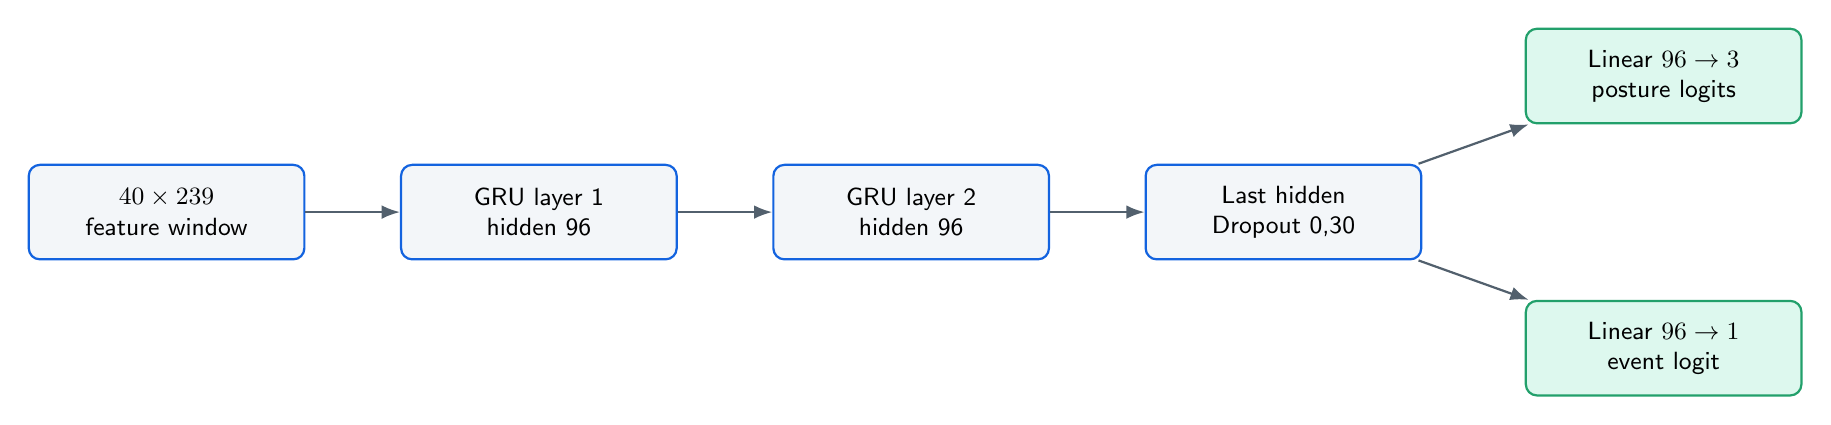
\begin{tikzpicture}[
  node distance=10mm and 12mm,
  box/.style={rounded corners,draw=fgBlue,fill=fgLight,minimum width=35mm,
    minimum height=12mm,align=center,font=\small\sffamily,thick},
  head/.style={box,draw=fgGreen,fill=fgMint},
  arrow/.style={-{Latex},thick,draw=fgGray}
]
\node[box] (x) {$40\times239$\\feature window};
\node[box,right=of x] (gru1) {GRU layer 1\\hidden 96};
\node[box,right=of gru1] (gru2) {GRU layer 2\\hidden 96};
\node[box,right=of gru2] (drop) {Last hidden\\Dropout 0,30};
\node[head,above right=5mm and 13mm of drop] (posture) {Linear $96\to3$\\posture logits};
\node[head,below right=5mm and 13mm of drop] (event) {Linear $96\to1$\\event logit};
\draw[arrow] (x)--(gru1);
\draw[arrow] (gru1)--(gru2);
\draw[arrow] (gru2)--(drop);
\draw[arrow] (drop)--(posture);
\draw[arrow] (drop)--(event);
\end{tikzpicture}}
\caption{Mô hình GRU đa nhiệm được dùng cho checkpoint hiện tại.}
\label{fig:model}
\end{figure}

Mô hình là GRU một chiều, hai tầng, hidden size 96, dropout 0,30. Hidden state
cuối cùng đi qua hai linear head:

\begin{align}
\mathbf{h}_t &= \mathrm{GRU}(\mathbf{X}_t),\\
\mathbf{z}^{posture}_t &= W_p\mathbf{h}_t+b_p,\\
z^{event}_t &= W_e\mathbf{h}_t+b_e,\\
\hat{p}^{event}_t &= \sigma(z^{event}_t).
\end{align}

Posture head có ba logit cho \code{UPRIGHT}, \code{TRANSITION}, \code{LYING};
event head có một logit nhị phân. Hai task chia sẻ encoder, nên thông tin tư thế
đóng vai trò regularization và giải thích cho dự đoán event.

\section{Hàm mất mát và mất cân bằng lớp}

Hàm mất mát tổng:

\[
\mathcal{L}=\mathcal{L}_{event}+\lambda_p\mathcal{L}_{posture},
\qquad \lambda_p=0,30.
\]

$\mathcal{L}_{posture}$ là weighted cross entropy; $\mathcal{L}_{event}$ là
binary cross entropy with logits với positive weight. Trên tập train hiện tại:

\begin{itemize}
  \item posture counts: 443 upright, 124 transition, 228 lying;
  \item event counts: 714 negative, 81 positive;
  \item posture weights: 0,4604; 1,6449; 0,8946;
  \item event positive weight: $714/81\approx8,8148$.
\end{itemize}

Việc đặt trọng số làm giảm xu hướng mô hình luôn đoán lớp phổ biến. AdamW dùng
learning rate $10^{-3}$, weight decay $10^{-4}$, batch size 32. Seed bằng 42 và
chế độ deterministic được lưu trong metadata.

\section{Thông số checkpoint thật}

\begin{table}[H]
\centering
\caption{Thông số checkpoint GRU tốt nhất của thí nghiệm.}
\begin{tabularx}{\textwidth}{p{5.4cm}Y}
\toprule
Thuộc tính & Giá trị \\
\midrule
Architecture & Causal GRU \\
Input size & 239 feature/frame \\
Window & 40 frame @ 20 FPS \\
Hidden size / layers & 96 / 2 \\
Dropout & 0,30 \\
Số tham số & 153.316, đều trainable \\
Thiết bị train & CUDA \\
Best epoch & 9 \\
Epoch đã chạy & 16/30, dừng sớm \\
Best validation loss & 0,35755 \\
Train / validation samples & 795 / 121 \\
\bottomrule
\end{tabularx}
\end{table}

\chapter{Huấn luyện, calibration và đánh giá}

\section{Quy trình huấn luyện}

Mỗi epoch chạy train với optimizer và validation không cập nhật gradient. Sau
mỗi epoch, hệ thống lưu \pathcode{last.pt}; nếu validation loss tốt hơn, lưu
\pathcode{best.pt}. Nếu không cải thiện trong bảy epoch liên tiếp, early stopping
dừng quá trình. Artifact gồm:

\begin{itemize}
  \item \pathcode{best.pt}, \pathcode{last.pt}: trọng số, optimizer, config;
  \item \pathcode{config.yaml}: cấu hình snapshot của experiment;
  \item \pathcode{metadata.json}: model spec, class weights, seed, provenance;
  \item \pathcode{history.csv}: loss/accuracy từng epoch;
  \item \pathcode{metrics.json}: metric validation;
  \item \pathcode{calibration.json}: threshold và đường cong threshold;
  \item \pathcode{test_metrics_calibrated.json}: kết quả test cuối.
\end{itemize}

\section{Hiệu chỉnh ngưỡng không chạm test}

Threshold mặc định 0,5 không nhất thiết tối ưu cho event. Hệ thống quét 101 giá
trị trên validation và chọn threshold theo event-level F1; tie-break lần lượt là
recall, precision và threshold nhỏ hơn. API calibration từ chối đường dẫn hoặc
metadata có nhãn \code{test}. Kết quả chọn $\tau=0,86$; threshold này được giữ
nguyên cho test.

\section{Metric theo frame và theo sự kiện}

Frame metrics xem từng cửa sổ là một mẫu. Event-level metrics gom các vùng dương
liên tục theo sequence, sau đó ghép một-một vùng dự đoán và vùng ground truth nếu
chúng giao nhau. Các công thức chính:

\[
P=\frac{TP}{TP+FP},\qquad
R=\frac{TP}{TP+FN},\qquad
F_1=\frac{2PR}{P+R}.
\]

False alarms/video bằng tổng false-positive event chia số video. Detection delay
là chênh lệch giữa thời điểm bắt đầu vùng dự đoán và vùng thật cho các event ghép
thành công.

\section{Kết quả test độc lập}

\begin{table}[H]
\centering
\caption{Kết quả thực tế trên 156 test windows thuộc 9 sequence có window hợp lệ.}
\begin{tabular}{lr}
\toprule
Metric & Giá trị \\
\midrule
Posture accuracy & 0,840 \\
Posture macro F1 & 0,615 \\
Frame event precision & 0,429 \\
Frame event recall & 1,000 \\
Frame event F1 & 0,600 \\
Event-level precision & 0,600 \\
Event-level recall & 1,000 \\
Event-level F1 & 0,750 \\
True / false / missed events & 3 / 2 / 0 \\
False alarms/video & 0,222 \\
\bottomrule
\end{tabular}
\end{table}

\begin{figure}[H]
\centering
\begin{tikzpicture}
\begin{axis}[
  ybar,bar width=13pt,width=0.9\textwidth,height=7cm,
  ymin=0,ymax=1.1,ymajorgrids=true,
  symbolic x coords={PostureAcc,PostureMacroF1,FrameP,FrameR,FrameF1,EventP,EventR,EventF1},
  xtick=data,xticklabel style={rotate=35,anchor=east,font=\small},
  ylabel={Giá trị},nodes near coords,nodes near coords style={font=\scriptsize},
  every axis plot/.append style={fill=fgBlue,draw=fgNavy}
]
\addplot coordinates {(PostureAcc,0.840) (PostureMacroF1,0.615)
 (FrameP,0.429) (FrameR,1.000) (FrameF1,0.600)
 (EventP,0.600) (EventR,1.000) (EventF1,0.750)};
\end{axis}
\end{tikzpicture}
\caption{Các metric chính của checkpoint sau calibration.}
\end{figure}

\begin{resultbox}[Cách diễn giải đúng]
Recall 1,0 trên test nhỏ nghĩa là không bỏ sót ba ground-truth event có thể đánh
giá trong split này; nó không chứng minh hệ thống không bỏ sót ngoài đời thực.
Precision 0,6 và 0,222 false alarm/video cho thấy vẫn có cảnh báo giả. Lớp
\code{TRANSITION} chỉ có 7 mẫu test và F1 bằng 0,10, là điểm yếu rõ ràng cần báo
cáo trung thực.
\end{resultbox}

\chapter{State machine xác minh té ngã}

\section{Tại sao cần state machine}

Neural network cho xác suất ở từng thời điểm nhưng cảnh báo là quyết định có
ngữ cảnh. State machine làm mượt xác suất, kiểm tra thời lượng và tạo một event
ID duy nhất. Nó giảm cảnh báo do spike ngắn và ngăn gửi Telegram lặp lại trên
nhiều frame \code{CONFIRMED\_FALL}.

\section{EMA xác suất}

Xác suất được làm mượt:

\[
\bar p_t=\alpha p_t+(1-\alpha)\bar p_{t-1},\qquad \alpha=0,40.
\]

Ngưỡng candidate trong cấu hình MVP là 0,70; ngưỡng high-confidence là 0,82.
Profile demo dùng ngưỡng xác nhận 0,86 để khớp threshold calibration.

\section{Các trạng thái}

\begin{figure}[H]
\centering
\resizebox{0.96\textwidth}{!}{%
\begin{tikzpicture}[
 state/.style={ellipse,draw=fgBlue,fill=fgLight,thick,minimum width=31mm,
   minimum height=13mm,align=center,font=\small\sffamily},
 alert/.style={state,draw=fgRed,fill=red!8},
 safe/.style={state,draw=fgGreen,fill=fgMint},
 arr/.style={-{Latex},thick,draw=fgGray},
 node distance=14mm and 18mm]
\node[safe] (normal) {NORMAL};
\node[state,right=of normal] (possible) {POSSIBLE\\FALL};
\node[state,right=of possible] (verify) {VERIFYING};
\node[alert,right=of verify] (confirmed) {CONFIRMED\\FALL};
\node[safe,below=of verify] (recovered) {RECOVERED};
\draw[arr] (normal)--node[above,font=\scriptsize]{vượt ngưỡng}(possible);
\draw[arr] (possible)--node[above,font=\scriptsize]{đủ thời gian}(verify);
\draw[arr] (verify)--node[above,font=\scriptsize]{nằm + bất động}(confirmed);
\draw[arr] (verify)--node[right,font=\scriptsize]{đứng lại}(recovered);
\draw[arr] (confirmed)--node[right,font=\scriptsize]{đứng lại}(recovered);
\draw[arr,bend left=35] (recovered) to node[below,font=\scriptsize]{hết cooldown}(normal);
\draw[arr,bend right=35] (possible) to node[below,font=\scriptsize]{tín hiệu giảm}(normal);
\end{tikzpicture}}
\caption{Luồng trạng thái xác minh sự kiện.}
\end{figure}

\begin{description}[style=nextline]
  \item[\code{NORMAL}] Không có candidate; risk thấp.
  \item[\code{POSSIBLE\_FALL}] EMA vượt ngưỡng candidate; bắt đầu đo thời gian.
  \item[\code{VERIFYING}] Tín hiệu tồn tại đủ lâu; theo dõi nằm, motion và hồi phục.
  \item[\code{CONFIRMED\_FALL}] Đã thấy high-confidence, nằm đủ lâu và bất động
  đủ lâu; risk cao, tạo event ID, lưu ảnh và gửi cảnh báo.
  \item[\code{RECOVERED}] Người đứng lại đủ lâu; ghi nhận self-recovery và chờ
  hết cooldown trước khi trở về normal.
\end{description}

\section{Đo bất động}

Với hai pose liên tiếp, hệ thống lấy median khoảng cách Euclid của các joint cùng
hợp lệ. Nếu motion không vượt 0,012 thì bắt đầu/tích lũy bất động. Nếu mất pose,
có ít hơn ba joint chung, hoặc gap lớn hơn một giây, bộ đếm bất động bị reset.
Cách làm bảo thủ này tránh xác nhận do camera không nhìn thấy người.

\section{Cấu hình MVP và cấu hình demo}

\begin{table}[H]
\centering
\caption{Khác biệt giữa profile thực tế và profile benchmark.}
\begin{tabular}{lrr}
\toprule
Tham số & \pathcode{mvp.yaml} & \pathcode{urfd_demo.yaml} \\
\midrule
Possible threshold & 0,70 & 0,70 \\
Confirm threshold & 0,82 & 0,86 \\
Candidate duration & 0,25 s & 0,10 s \\
Lying duration & 2,00 s & 0,50 s \\
Inactive duration & 8,00 s & 0,00 s \\
Recovery upright & 1,50 s & 1,00 s \\
Cooldown & 20,00 s & 5,00 s \\
\bottomrule
\end{tabular}
\end{table}

URFD clip chỉ dài vài giây, nên profile demo bỏ yêu cầu bất động tám giây. Khi
demo webcam trong điều kiện thực tế, nên dùng \pathcode{configs/mvp.yaml} hoặc
tinh chỉnh có kiểm chứng, không dùng shortcut benchmark để tuyên bố an toàn.

\chapter{Suy luận video và webcam}

\section{Video inference}

Video được đọc bằng OpenCV, resample về target FPS, chạy pose và đưa frame hợp
lệ/placeholder vào sequence buffer. Khi đủ 40 frame và tới stride, model tạo
prediction. Kết quả được vẽ skeleton, state, posture và fall probability lên
video; event được xuất JSON.

Luồng web lưu upload tạm dưới \pathcode{runtime/uploads}, chạy inference trong
threadpool, tạo video annotated và JSON dưới \pathcode{runtime/results}, rồi xóa
upload gốc. Khi vừa xác nhận ngã, hệ thống trích đúng frame theo timestamp từ
video annotated và lưu JPEG tại \pathcode{runtime/results/snapshots}.

\section{Webcam realtime}

Webcam dùng cùng feature/model/state machine với video. Network Telegram chạy
trong một worker nền duy nhất để không chặn vòng lặp camera. Hệ thống gửi theo
cờ ``vừa xác nhận'' trong metadata, không phải chỉ kiểm tra state; nhờ đó một
event chỉ gửi một lần dù trạng thái xác nhận còn tồn tại qua nhiều frame.

\begin{figure}[H]
\centering
\includegraphics[width=0.72\textwidth]{demo_videos/telegram_samples/01_FALL_CONFIRMED_snapshot.jpg}
\caption{Snapshot annotated được trích tại thời điểm xác nhận fall trong video demo.}
\label{fig:snapshot}
\end{figure}

\section{Ba chế độ demo}

\begin{table}[H]
\centering
\caption{Mục đích của các giao diện demo.}
\begin{tabularx}{\textwidth}{p{3.5cm}p{3.8cm}Y}
\toprule
Chế độ & Nguồn vào & Mục đích \\
\midrule
CLI video & File cục bộ & Debug pipeline và xuất annotated video/JSON \\
CLI camera & Webcam/USB camera & Trình diễn phát hiện trực tiếp trên máy tính \\
Dashboard web & File upload vào localhost & Giao diện dễ dùng, lịch sử, metrics, feedback \\
Skeleton API & Tọa độ 33 khớp & Tích hợp từ hệ thống pose bên ngoài; Telegram text-only \\
\bottomrule
\end{tabularx}
\end{table}

\chapter{Backend, dashboard và lưu trữ}

\section{FastAPI}

FastAPI cung cấp validation theo type hint và OpenAPI/Swagger UI tự động
\cite{fastapi}. Ứng dụng chạy mặc định tại \url{http://127.0.0.1:8000}; đây là
localhost, không tự tải video lên Internet.

\begin{longtable}{p{2.1cm}p{5.1cm}p{7.2cm}}
\caption{Các endpoint chính.}\\
\toprule
Method & Endpoint & Chức năng \\
\midrule
\endfirsthead
\toprule
Method & Endpoint & Chức năng \\
\midrule
\endhead
GET & \pathcode{/health} & Trạng thái dịch vụ, database và model \\
GET & \pathcode{/v1/model} & Metadata model, window, FPS và output \\
POST & \pathcode{/v1/predict/skeleton} & Dự đoán từ chuỗi 33 landmarks \\
POST & \pathcode{/v1/predict/video} & Upload, phân tích video, tạo artifact \\
GET & \pathcode{/v1/events} & Danh sách sự kiện có filter/pagination \\
GET & \pathcode{/v1/events/{event_id}} & Chi tiết một event \\
POST & \pathcode{/v1/events/{event_id}/feedback} & Gán nhãn review đúng/sai \\
GET & \pathcode{/v1/metrics/summary} & Tổng hợp số event/feedback \\
\bottomrule
\end{longtable}

Upload chỉ nhận các phần mở rộng video cho phép, giới hạn mặc định 250 MB và
thời lượng xử lý tối đa năm phút. Tên file server dùng UUID thay vì tên do người
dùng cung cấp để tránh ghi đè/path traversal.

\section{SQLite event store}

Mỗi event có các trường: event ID, state, risk, timestamp, camera ID, person ID,
source, fall probability, inactive seconds, self-recovery, evidence, metadata,
feedback và thời gian tạo/cập nhật. \code{UPSERT} cho phép một event chuyển từ
confirmed sang recovered mà không tạo bản ghi trùng.

Feedback gồm label, ghi chú, reviewer và thời gian. Đây là nền tảng để thu thập
false alarm có kiểm duyệt và tái huấn luyện về sau.

\section{Dashboard}

Dashboard HTML/CSS/JavaScript không cần build frontend riêng. Người dùng thả
video, nhập Camera ID/Person ID, chọn cờ URFD preview, nhấn phân tích và xem:

\begin{itemize}
  \item trạng thái cuối, risk, xác suất và timeline;
  \item video annotated và JSON kết quả;
  \item lịch sử sự kiện từ SQLite;
  \item số liệu tổng hợp và feedback review.
\end{itemize}

Camera ID chỉ là nhãn nguồn, ví dụ \code{CAM-DEMO-01}, không phải index webcam.
Person ID có thể để trống nhưng hữu ích khi lọc lịch sử.

\chapter{Cảnh báo Telegram và webhook}

\section{Luồng Telegram}

Khi state machine tạo \code{just\_confirmed=True}:

\begin{enumerate}
  \item event ID được thêm vào set chống trùng trước khi scheduling;
  \item snapshot annotated được lưu cục bộ;
  \item event đã lưu SQLite (có \code{created\_at}) được format thành tiếng Việt;
  \item ảnh JPEG và caption được gửi qua phương thức \code{sendPhoto} của
  Telegram Bot API; nếu ảnh lỗi, hệ thống chuyển sang \code{sendMessage};
  \item timeout/lỗi mạng được trả thành kết quả có cấu trúc, không làm inference
  dừng.
\end{enumerate}

Telegram Bot API là HTTP interface và yêu cầu \code{chat\_id} là định danh cuộc
trò chuyện đích \cite{telegramapi}. Bot username hoặc link \code{t.me/...} không
phải Chat ID cá nhân. Người nhận phải mở bot và gửi \code{/start} trước khi bot
có thể gửi tin.

\section{Bảo mật token}

Token được đọc từ biến môi trường hoặc file \pathcode{.env} cục bộ. File này
nằm trong \pathcode{.gitignore}; biến đã có trong PowerShell được ưu tiên hơn
\pathcode{.env}. Token không được đưa vào CLI argument, \code{repr}, log hoặc
error message. Bất kỳ token nào đã dán vào chat/Git/ảnh chụp phải được revoke và
tạo lại bằng BotFather.

Các biến hỗ trợ:

\begin{lstlisting}
FALLGUARD_TELEGRAM_BOT_TOKEN=
FALLGUARD_TELEGRAM_CHAT_ID=
FALLGUARD_TELEGRAM_CHAT_IDS=
FALLGUARD_TELEGRAM_ENABLED=true
FALLGUARD_TELEGRAM_TIMEOUT_SECONDS=8
\end{lstlisting}

\section{Webhook}

Ngoài Telegram, hệ thống có thể POST event JSON đến dịch vụ khác. URL lấy từ
\path{FALLGUARD_ALERT_WEBHOOK} hoặc \path{FALLGUARD_WEBHOOK_URL}; secret
tùy chọn dùng cho xác thực. Webhook và Telegram dùng cùng logic dedupe nhưng là
hai adapter độc lập.

\section{Quyền riêng tư}

Web dashboard chạy localhost, nhưng ảnh gửi Telegram sẽ rời máy tính và đi vào
hạ tầng Telegram. Chỉ bật tính năng khi người xuất hiện trong video đồng ý;
giới hạn Chat ID; bảo vệ cả snapshot cục bộ; có lịch xóa dữ liệu; không đặt
camera ở khu vực riêng tư.

\chapter{Hướng dẫn chạy dự án từ đầu}

\section{Yêu cầu}

\begin{itemize}
  \item Windows 10/11, PowerShell và kết nối Internet cho bước tải dữ liệu/model;
  \item webcam nếu demo realtime;
  \item GPU CUDA là tùy chọn, CPU vẫn chạy được;
  \item đủ dung lượng: preview nhẹ hơn nhiều so với profile RGB đầy đủ.
\end{itemize}

\section{Bước 1 - Cài môi trường}

Tại thư mục gốc repository:

\begin{lstlisting}[language=bash]
Set-ExecutionPolicy -Scope Process Bypass
.\scripts\bootstrap.ps1
.\.venv\Scripts\Activate.ps1
fallguard doctor
\end{lstlisting}

Bootstrap tải \code{uv} và CPython 3.12 vào workspace, tạo \pathcode{.venv}, đọc
\pathcode{uv.lock} và cài các dependency. \code{fallguard doctor} kiểm tra cấu
hình, package, accelerator và storage.

\section{Bước 2 - Smoke test không cần dataset công khai}

\begin{lstlisting}[language=bash]
fallguard demo --epochs 3
\end{lstlisting}

Lệnh tạo skeleton synthetic, materialize window, train vài epoch và evaluate.
Nếu bước này chạy được, toolchain PyTorch/pipeline cơ bản đã hoạt động.

\section{Bước 3 - Tải URFD}

Đọc giấy phép trước, sau đó:

\begin{lstlisting}[language=bash]
fallguard data download-urfd `
  --selection full `
  --profile preview `
  --accept-license `
  --no-extract
\end{lstlisting}

Muốn kiểm tra nhanh, thay \code{full} bằng \code{smoke}. Không nên xóa file
\code{.part} khi download gián đoạn vì downloader có thể resume.

\section{Bước 4 - Trích pose và tạo window}

\begin{lstlisting}[language=bash]
fallguard data prepare-urfd --source preview
fallguard data validate
\end{lstlisting}

Kết quả quan trọng:

\begin{lstlisting}
data/interim/urfd_preview/poses/*.npz
data/manifests/urfd_preview_sequences.csv
data/processed/urfd_preview/windows_train.npz
data/processed/urfd_preview/windows_validation.npz
data/processed/urfd_preview/windows_test.npz
\end{lstlisting}

\section{Bước 5 - Train}

\begin{lstlisting}[language=bash]
fallguard train `
  --data-dir data/processed/urfd_preview `
  --output artifacts/urfd_preview_gru
\end{lstlisting}

Theo dõi \pathcode{history.csv}. Không chọn model bằng test result; checkpoint
tốt nhất chỉ dựa trên validation loss.

\section{Bước 6 - Calibration}

\begin{lstlisting}[language=bash]
fallguard calibrate `
  artifacts/urfd_preview_gru/best.pt `
  --validation-data data/processed/urfd_preview `
  --output artifacts/urfd_preview_gru/calibration.json
\end{lstlisting}

\section{Bước 7 - Đánh giá test}

\begin{lstlisting}[language=bash]
fallguard evaluate `
  artifacts/urfd_preview_gru/best.pt `
  --data-dir data/processed/urfd_preview `
  --split test `
  --calibration artifacts/urfd_preview_gru/calibration.json `
  --output artifacts/urfd_preview_gru/test_metrics_calibrated.json
\end{lstlisting}

\section{Bước 8 - Video inference}

Video bình thường:

\begin{lstlisting}[language=bash]
fallguard infer video my-video.mp4 `
  --checkpoint artifacts/urfd_preview_gru/best.pt
\end{lstlisting}

Video preview URFD phải bật crop:

\begin{lstlisting}[language=bash]
fallguard infer video demo_videos/01_FALL_CONFIRMED_URFD_fall-19.mp4 `
  --checkpoint artifacts/urfd_preview_gru/best.pt `
  --config configs/urfd_demo.yaml `
  --urfd-preview
\end{lstlisting}

\section{Bước 9 - Webcam realtime}

\begin{lstlisting}[language=bash]
fallguard infer camera `
  --source 0 `
  --checkpoint artifacts/urfd_preview_gru/best.pt `
  --config configs/mvp.yaml `
  --camera-id CAM-DEMO-01 `
  --person-id USER-001 `
  --telegram
\end{lstlisting}

Nhấn \code{Q} hoặc \code{Esc} để dừng. Nếu máy có nhiều camera, thử
\code{--source 1}. Không dùng một người lớn tuổi hoặc người có bệnh nền để mô
phỏng ngã; demo an toàn trên nệm và có người hỗ trợ.

\section{Bước 10 - Dashboard web}

Khởi động nhanh đúng profile demo:

\begin{lstlisting}[language=bash]
powershell -ExecutionPolicy Bypass `
  -File .\demo_videos\START_WEB_DEMO.ps1
\end{lstlisting}

Hoặc chạy trực tiếp:

\begin{lstlisting}[language=bash]
fallguard serve `
  --checkpoint artifacts/urfd_preview_gru/best.pt `
  --config configs/urfd_demo.yaml `
  --open
\end{lstlisting}

Mở các địa chỉ sau trong trình duyệt:
\begin{itemize}
  \item dashboard: \url{http://127.0.0.1:8000};
  \item tài liệu Swagger: \url{http://127.0.0.1:8000/docs}.
\end{itemize}
Với file có tên chứa \code{URFD}, dashboard tự bật crop preview; video điện
thoại/webcam bình thường không bật tùy chọn này.

\section{Bước 11 - Telegram}

\begin{lstlisting}[language=bash]
powershell -ExecutionPolicy Bypass `
  -File .\scripts\configure_telegram.ps1
\end{lstlisting}

Script yêu cầu token mới nhập ẩn, hướng dẫn \code{/start}, discovery Chat ID,
lưu \pathcode{.env} và gửi ảnh mẫu. Có thể kiểm tra lại:

\begin{lstlisting}[language=bash]
fallguard telegram test `
  --snapshot .\demo_videos\telegram_samples\01_FALL_CONFIRMED_snapshot.jpg
\end{lstlisting}

Nếu cấu hình khi server đang chạy, phải dừng bằng \code{Ctrl+C} và khởi động lại
để process nạp \pathcode{.env} mới.

\section{Bước 12 - Test và lint}

\begin{lstlisting}[language=bash]
pytest -q
ruff check .
\end{lstlisting}

Tại thời điểm hoàn thiện Telegram/dotenv, toàn bộ suite có 77 test pass. Test
bao phủ downloader, parser, split, preprocessing, model shape, training smoke,
calibration, state machine, video, API, SQLite, evidence và Telegram mock.

\chapter{Kịch bản demo bảo vệ đồ án}

\section{Demo web ổn định}

\begin{enumerate}
  \item Chạy \pathcode{START_WEB_DEMO.ps1}.
  \item Chọn \pathcode{01_FALL_CONFIRMED_URFD_fall-19.mp4}.
  \item Xác nhận cờ ``Video mẫu URFD'' đang bật.
  \item Nhập \code{CAM-DEMO-01}, nhấn phân tích.
  \item Trình bày video annotated, state \code{CONFIRMED\_FALL}, probability,
  lịch sử SQLite và tin Telegram.
  \item Chọn một ADL normal để chứng minh không phải video nào cũng cảnh báo.
\end{enumerate}

Chín mẫu gồm hai confirmed fall, các ADL normal/hard negative và các case
\code{VERIFYING}. Case biên rất hữu ích để giải thích hệ thống biết từ chối khi
chưa đủ bằng chứng.

\section{Demo realtime}

Đặt webcam sao cho thấy toàn thân, camera cố định, đủ sáng và nền không quá rối.
Chờ buffer đủ hai giây. Người demo có thể mô phỏng chuyển từ đứng sang ngồi/nằm
trên nệm, nhưng phải ưu tiên an toàn. Với profile MVP, cần nằm và bất động đủ
thời gian; vì vậy demo realtime dài hơn video benchmark.

\section{Thông điệp trình bày}

Một flow thuyết trình ngắn:

\begin{enumerate}
  \item Pixel được đổi thành skeleton 33 khớp để giảm phụ thuộc ngoại hình.
  \item 40 frame tạo lịch sử hai giây, GRU học động học chứ không nhìn một ảnh.
  \item Hai head phân biệt posture và event.
  \item State machine xác minh nằm/bất động và chống cảnh báo giả.
  \item Event được lưu, có snapshot và gửi Telegram để người chăm sóc kiểm tra.
\end{enumerate}

\chapter{Hạn chế, rủi ro và hướng phát triển}

\section{Hạn chế dữ liệu và mô hình}

\begin{itemize}
  \item URFD nhỏ, fall được diễn, không đại diện đầy đủ người cao tuổi thực tế.
  \item Split hiện tại cross-sequence, chưa chứng minh tổng quát cross-subject.
  \item Transition ít mẫu và metric thấp.
  \item Một camera RGB khó xử lý che khuất, thiếu sáng, góc nhìn lạ hoặc camera rung.
  \item Pipeline không có multi-person tracking; người nổi bật nhất có thể thay đổi.
  \item Nằm chủ động, quỳ, tập thể dục, ngồi nhanh hoặc xe lăn có thể tạo false alarm.
\end{itemize}

\section{Hạn chế đánh giá}

Test chỉ có chín sequence tạo được window đánh giá và ba ground-truth event ở
metric event-level. Khoảng tin cậy chưa được báo cáo. Detection delay 0 trong
artifact frame-level không bao gồm toàn bộ thời gian hậu kiểm 8 giây của profile
MVP. Do đó không nên dùng metric này để tuyên bố cảnh báo y tế tức thì.

\section{An toàn và đạo đức}

\begin{itemize}
  \item Có consent rõ ràng; ưu tiên lưu skeleton thay video gốc khi có thể.
  \item Mã hóa Person ID, hạn chế quyền xem SQLite/snapshot và đặt retention.
  \item Không gửi ảnh cho Chat ID ngoài nhóm chăm sóc được ủy quyền.
  \item Không tự động gọi cấp cứu chỉ dựa trên một model prototype.
  \item Cho phép người kiểm duyệt feedback false alarm/missed event.
\end{itemize}

\section{Lộ trình phát triển}

\begin{enumerate}
  \item Thu tập dữ liệu webcam tự quay với consent: đứng, đi, ngồi, cúi, nằm chủ
  động, chuyển tư thế nhanh, ánh sáng/góc nhìn khác nhau.
  \item Split theo người khi có subject ID; đánh giá domain gap URFD $\to$ webcam.
  \item Ablation: tọa độ; +velocity; +geometry; có/không state machine.
  \item So sánh GRU, LSTM, TCN trên cùng split và compute budget.
  \item Quét inactivity 2/4/6/8 giây để đo trade-off false alarm và latency.
  \item Thêm person tracking và hỗ trợ nhiều người.
  \item Quantization/ONNX để giảm latency CPU; benchmark FPS, P50/P95 và RAM.
  \item Dashboard realtime qua WebSocket, phân quyền người dùng và audit log.
  \item Escalation: Telegram lần một, caregiver xác nhận, rồi mới gọi dịch vụ khác.
\end{enumerate}

\chapter{Kết luận}

FallGuard AI là một prototype hoàn chỉnh từ dữ liệu đến ứng dụng. Thiết kế chủ
đạo là biến video thành pose, biến pose thành đặc trưng thời gian, dùng GRU đa
nhiệm để dự đoán posture và fall-event, rồi dùng state machine để chuyển dự đoán
thành sự kiện có thể giải thích. Hệ thống đã có checkpoint và kết quả đánh giá
thật, chạy được trên video/webcam, cung cấp API/dashboard, lưu SQLite và gửi
Telegram kèm ảnh.

Điểm quan trọng khi trình bày không phải là khẳng định hệ thống đã đủ dùng trong
y tế, mà là chứng minh một quy trình kỹ thuật đúng: dữ liệu có nguồn và giấy
phép; nhãn có provenance; split tránh leakage; threshold không tối ưu trên test;
runtime nhân quả; cảnh báo có hậu kiểm; metric và giới hạn được báo cáo trung
thực. Đây là nền móng tốt để mở rộng thành nghiên cứu cross-subject, đa dữ liệu
và thử nghiệm thực địa trong giai đoạn tiếp theo.

\appendix
\chapter{Bảng tham số cấu hình}

\begin{longtable}{p{5.6cm}p{2.5cm}p{6.2cm}}
\caption{Các tham số chính của cấu hình MVP.}\\
\toprule
Khóa & Giá trị & Ý nghĩa \\
\midrule
\endfirsthead
\toprule
Khóa & Giá trị & Ý nghĩa \\
\midrule
\endhead
\pathcode{project.seed} & 42 & Seed tái lập \\
\pathcode{project.device} & auto & CUDA nếu có, nếu không CPU \\
\pathcode{data.target_fps} & 20 & Tần số xử lý \\
\pathcode{data.window_size} & 40 & Số frame trong một window \\
\pathcode{data.stride} & 5 & Khoảng cách hai window \\
\path{data.max_interpolation_gap} & 3 & Gap landmark tối đa được nội suy \\
\pathcode{data.min_pose_visibility} & 0,35 & Ngưỡng landmark hợp lệ \\
\path{features.normalize_center} & hip & Tâm chuẩn hóa \\
\pathcode{features.normalize_scale} & torso & Scale theo thân \\
\pathcode{model.architecture} & gru & Encoder chính \\
\pathcode{model.hidden_size} & 96 & Hidden dimension \\
\pathcode{model.num_layers} & 2 & Số recurrent layer \\
\pathcode{model.dropout} & 0,30 & Regularization \\
\pathcode{training.batch_size} & 32 & Batch train \\
\pathcode{training.epochs} & 30 & Epoch tối đa \\
\pathcode{training.learning_rate} & 0,001 & Learning rate AdamW \\
\pathcode{training.patience} & 7 & Early stopping patience \\
\path{event_detection.ema_alpha} & 0,40 & Mức làm mượt probability \\
\path{event_detection.inactive_seconds} & 8,0 & Thời gian bất động cần xác minh \\
\pathcode{api.max_upload_mb} & 250 & Kích thước upload tối đa \\
\bottomrule
\end{longtable}

\chapter{Xử lý lỗi thường gặp}

\begin{longtable}{p{5cm}p{9.3cm}}
\caption{Troubleshooting nhanh.}\\
\toprule
Hiện tượng & Nguyên nhân và cách xử lý \\
\midrule
\endfirsthead
\toprule
Hiện tượng & Nguyên nhân và cách xử lý \\
\midrule
\endhead
Không mở được camera & Thử \code{--source 1}; đóng Zoom/Teams; kiểm tra quyền camera. \\
Camera chạy nhưng không predict & Chờ đủ 40 frame; bảo đảm thấy toàn thân và đủ sáng. \\
Video URFD hiển thị depth+RGB & Bật \code{--urfd-preview} hoặc checkbox tương ứng. \\
Video thường bị crop mất nửa & Tắt URFD preview cho video điện thoại/webcam. \\
Telegram 400 chat not found & Chat ID sai; gửi \code{/start}, chạy discover và dùng ID số chính xác. \\
Telegram 401/404 & Token sai, đã revoke hoặc process đang giữ token cũ; tạo token mới và restart server. \\
Telegram 409 getUpdates & Bot đang có webhook/poller khác; dừng process hoặc xóa webhook có chủ đích. \\
Không có ảnh Telegram & Skeleton API không có pixel hoặc snapshot lỗi; hệ thống fallback text. \\
Port 8000 bận & Dừng server cũ bằng \code{Ctrl+C} hoặc chọn port khác. \\
CUDA không dùng được & Chạy \code{fallguard doctor}; hệ thống có thể fallback CPU. \\
\bottomrule
\end{longtable}

\chapter{Câu hỏi bảo vệ gợi ý}

\begin{description}[style=nextline]
  \item[Tại sao không dùng YOLO để nhận diện người nằm?]
  Một bounding box hoặc class trên một frame không thể hiện quá trình chuyển từ
  đứng sang ngã. Pose + temporal model mô tả động học; state machine xác minh
  sau ngã. YOLO vẫn có thể bổ sung cho person detection/tracking nhưng không thay
  thế toàn bộ bài toán thời gian.

  \item[Tại sao dùng GRU?]
  GRU phù hợp chuỗi ngắn, ít tham số hơn LSTM, chạy causal và đủ nhẹ cho webcam.
  Repository vẫn có LSTM/TCN để so sánh khoa học.

  \item[Tại sao cần hai head?]
  Posture là nhãn có sẵn và giải thích trạng thái hình học; event là câu hỏi theo
  thời gian. Multi-task giúp encoder học cả tư thế lẫn diễn biến.

  \item[Tại sao recall cao nhưng precision thấp?]
  Class fall hiếm và mục tiêu ưu tiên không bỏ sót làm model nhạy. State machine,
  calibration và dữ liệu hard-negative được dùng để giảm false alarm, nhưng test
  vẫn cho thấy hai false-positive event.

  \item[Web có gửi video lên Internet không?]
  Không khi chạy ở \code{127.0.0.1}; browser gửi file cho FastAPI trên cùng máy.
  Telegram là ngoại lệ: snapshot được tải lên Telegram khi bật cảnh báo.

  \item[Metric hiện tại có đủ triển khai thực tế không?]
  Không. Cần dữ liệu người thật có consent, split theo người, kiểm thử nhiều góc
  camera, confidence interval, latency và false alarms/hour trước khi cân nhắc
  pilot thực địa.
\end{description}

\begin{thebibliography}{9}
\bibitem{urfdpaper}
Bogdan Kwolek và Michal Kępski,
``Human fall detection on embedded platform using depth maps and wireless
accelerometer,'' \textit{Computer Methods and Programs in Biomedicine},
117(3), 489--501, 2014. DOI:
\url{https://doi.org/10.1016/j.cmpb.2014.09.005}.

\bibitem{urfdsite}
University of Rzeszów, ``UR Fall Detection Dataset,''
\url{https://fenix.ur.edu.pl/~mkepski/ds/uf.html}, truy cập tháng 09/2026.

\bibitem{mediapipepose}
Google AI Edge, ``Pose landmark detection guide,''
\url{https://developers.google.com/edge/mediapipe/solutions/vision/pose_landmarker},
truy cập tháng 09/2026.

\bibitem{fastapi}
FastAPI, ``Tutorial - User Guide,''
\url{https://fastapi.tiangolo.com/tutorial/}, truy cập tháng 09/2026.

\bibitem{telegramapi}
Telegram, ``Telegram Bot API,''
\url{https://core.telegram.org/bots/api}, truy cập tháng 09/2026.
\end{thebibliography}

\end{document}
